% !TEX TS-program = pdflatex   
\documentclass[runningheads,12pt]{article} 
\usepackage{graphicx}
\usepackage{color,url}
\usepackage{mdframed}%put frame around text or a table
\usepackage{framed}
\usepackage{pdfpages}% Import pdf
\usepackage{soul}% Highlight
\usepackage{fancyvrb}

\usepackage{sty/bsymb} %% Event-B symbols
\usepackage{sty/eventB} %% REQ and ENV
\usepackage{sty/b2latex}% Importing from Rodin
\usepackage{sty/calculation} % Calculational proofs
\newcommand{\term}[1]{\textit{#1}}

\usepackage{amsmath}

\usepackage{fancyhdr,lastpage}
\lhead{\rm Greatest Common Divider in Eiffel}
\rhead {\rm Page \thepage~of \pageref{LastPage}}
\lfoot{}\cfoot{}\rfoot{}
\pagestyle{fancy}

% Listings needs package courier
\usepackage{listings} % Needs 
\usepackage{courier}
% Inline Eiffel Code
\newcommand{\e}[1]{\lstinline[language=eiffel]|#1|}

%Symbols
\def\Fl{\mathbb{F}}
\def\Rl{\mathbb{R}}
\def\Nl{\mathbb{N}}
\def\Bl{\mathbb{B}}
\def\St{\mathbb{S}}

\usepackage{stmaryrd}
\def\b{\llbracket \rrbracket}
\def\a{\rightarrow}


\begin{document}

\title{Greatest Common Divider (Eiffel)}
\author{JSO}
\date{19 June 2020}

\maketitle
\tableofcontents

\section{Formal Methods}

In mathematics, the Euclidean algorithm is an efficient method for computing the greatest common divisor (GCD) of two integers, the largest number that divides them both without a remainder. It is named after the ancient Greek mathematician Euclid, who first described it in his Elements (c. 300 BC). It is used in cryptographic computations to ensure the security of a variety of systems (\textit{Wikipedia}). 

\begin{quote}
Cybersecurity is everyone’s problem. The target may be the electric grid, government systems storing sensitive personnel data, intellectual property in the defense industrial base, or banks and the financial system. Adversaries range from small-time criminals to nation states and other determined opponents who will explore an ingenious range of attack strategies. And the damage may be tallied in dollars, in strategic advantage, or in human lives. Systematic, secure system design is urgently needed, and we believe that rigorous formal methods are essential for substantial improvements.

Formal methods enable reasoning from logical or mathematical specifications of the behaviors of computing devices or processes; they offer rigorous proofs that all system behaviors meet some desirable property. They are crucial for security goals, because they can show that no attack strategy in a class of strategies will cause a system to misbehave. Without requiring piecemeal enumeration, they rule out a range of attacks. They offer other benefits too: Formal specifications tell an implementer unambiguously what to produce, and they tell the subsequent user or integrator of a component what to rely on it to do. Since many vulnerabilities arise from misunderstandings and mismatches as components are integrated, the payoff from rigorous interface specifications is large.\footnote{%
\textit{Report on the NSF Workshop on Formal Methods for Security}, 2016, \url{https://arxiv.org/pdf/1608.00678.pdf}.}
\end{quote}

\section{Using Formal Methods to Verify Euclid's algorithm}

\noindent To understand the use of formal methods, let's look at a simple example. In Fig.~\ref{fig:gcd-c}, Euclid's algorithm is implemented in Golang.\footnote{%
Try it at \url{https://play.golang.org}.} 

\begin{figure}[!htb]
\begin{framed}
\begin{Verbatim}[fontsize=\small]
// golang
package main

import (
	"fmt"
)

// greatest common divisor (GCD) via Euclidean algorithm
// use only addition and subtraction 
func gcd(m, n int) int {
	x := m
	y := n
	for x != y {		// while loop
		if x < y {
			y = y - x
		} else {
			x = x - y
		}
	}
	return x
}

func main() {
	fmt.Println(gcd( 111, 259))
	fmt.Println(gcd(-111, 259))
}	
\end{Verbatim}
\end{framed}
The statement \textcolor{red}{\e{fmt.Println(gcd(-111, 259))}} is non-terminating. One might add an assert or defensive programming, neither of which is ideal. 
\caption{GCD implemented in Go}
\label{fig:gcd-c}
\noindent\rule{\textwidth}{0.5pt}
\end{figure}

%%%%%%%%%%%%%

\subsection{Testing can show the presence of bugs, but not their absence}

There is a while loop in the code of Fig.~\ref{fig:gcd-c}. How sure are we that this implementation always terminates? If it does terminate, how do we know it always terminates with the correct result?

\begin{figure*}[hbt]
  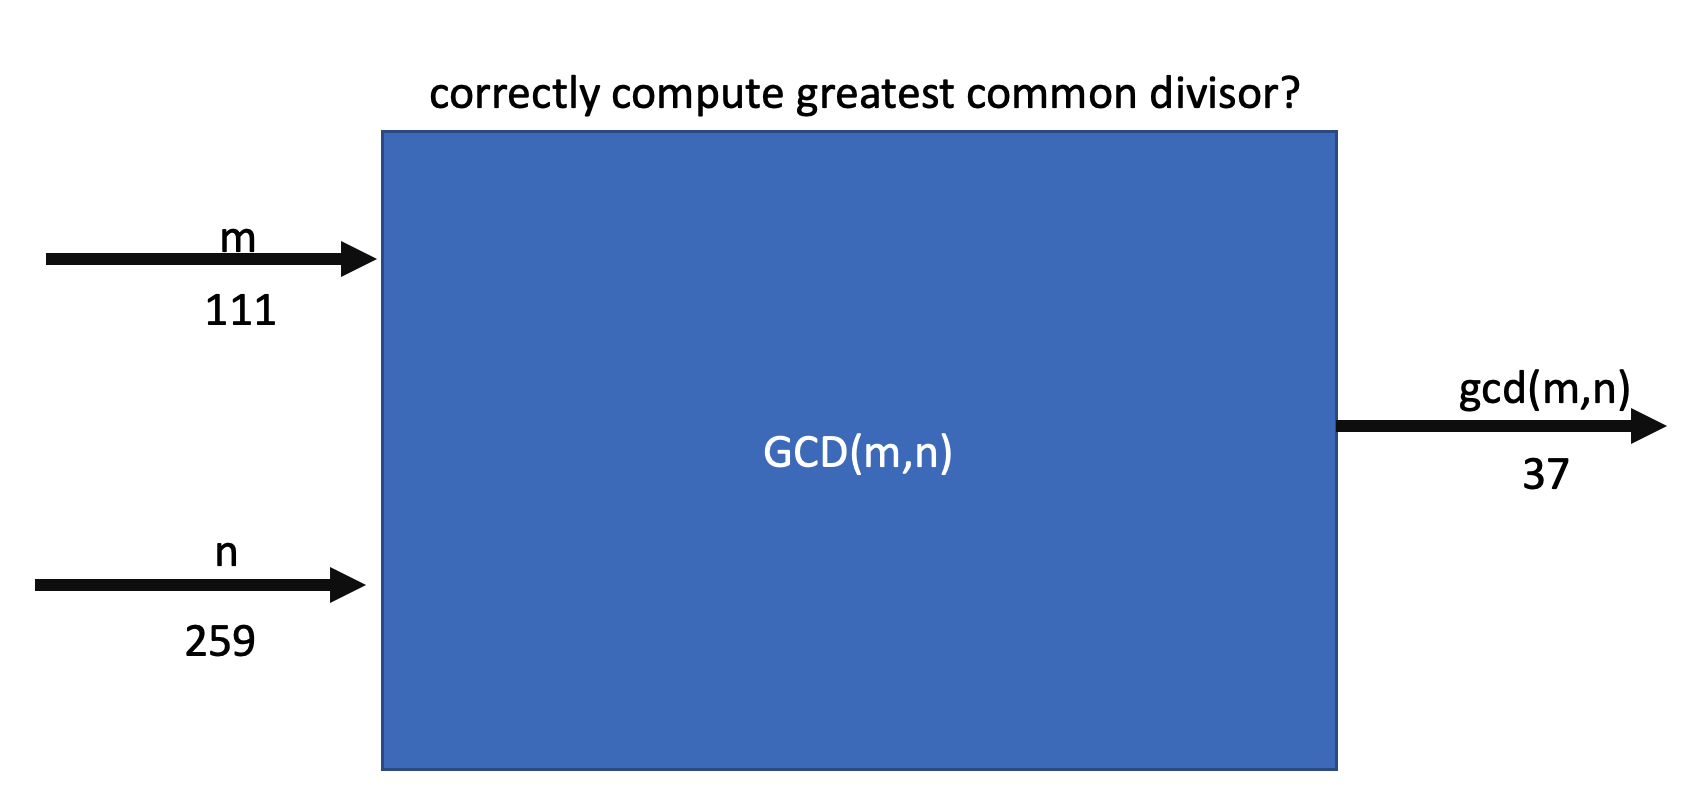
\includegraphics[width=0.8\textwidth]{images/gcd.png}
\end{figure*}


We can test the $gcd(m,n)$ subroutine. For example, we can provide inputs $m := 111$ and $n := 259$, and then we can check if the output is $gcd(111,259) = 37$. 

If we discover an an error in the code, then we can fix it. But here is the concern with testing alone: \textit{Dijkstra}: ``testing can show the presence of bugs, but not their absence". 

\begin{itemize}
  \item It does not matter how many tests we run, we can never exhaustively check the correctness of the algorithm. There are just too many combinations of inputs!
  \item To write a test, we also need to (manually?) compute the answer, a time consuming process. For example, to test gcd(111,259), we had to first manually compute the GCD by hand.\footnote{GCD is built-in in most programming languages. But we are assuming that, for the sake of illustration, that we are computing a new function, one for which there is no oracle.}
\end{itemize}

The earlier NSF report perhaps words it too strongly, but there is more than a grain of truth to it. 

\begin{quote}
Formal methods are the only reliable way to achieve security and privacy in computer systems. Formal methods, by modeling computer systems and adversaries, can prove that a system is immune to entire classes of attacks (provided the assumptions of the models are satisfied). By ruling out entire classes of potential attacks, formal methods offer an alternative to the “cat and mouse” game between adversaries and defenders of computer systems.

Formal methods can have this effect because they apply a scientific method. They provide scientific foundations in the form of precise adversary and system models, and derive cogent conclusions about the possible behaviors of the system as the adversary interacts with it. This is a central aspect of providing a science of security.
\end{quote}

For a formal proof Euclid's algorithm in TLA+, see \url{https://lamport.azurewebsites.net/pubs/euclid.pdf}.  Tools such as TLA+ has been used at Amazon, Microsoft and elsewhere. 

\section{Correctness needs a Specification}
%%%%%%%%%%%%%%%%%%%%%%%%%%%%%%%%%%%%%%%%%%%%

To judge whether code is correct, we need a \textbf{specification}---this is something different from the Go \textbf{implementation} in Fig.~\ref{fig:gcd-c}. A specification is the software engineering equivalent of blue-prints in other engineering disciplines.

\begin{quote}

Our recommendations are threefold, ... First, computer science majors, many of whom will be the designers and implementers of next-generation systems, should get a grounding in logic, ... “To designers of complex systems, the need for formal specs should be as obvious as the need for blueprints of a skyscraper. (Lesley Lamport) 

The methods, tools, and materials for educating students about ``formal specs" are ready for prime time. Mechanisms such as ``design by contract," now available in mainstream programming languages, should be taught as part of introductory programming, as is done in the introductory programming language sequence at Carnegie Mellon University. $\cdots$ We are failing our computer science majors if we do not teach them about the value of formal specifications.\footnote{%
``Teach Foundational Language Principles", Thomas Ball and Benjamin Zorn , \textit{Communications of the ACM}, May 2015, Vol. 58 No. 5, Pages 30-31. \url{https://cacm.acm.org/magazines/2015/5/186023-teach-foundational-language-principles/fulltext}. 

Thomas Ball (tball@microsoft.com) is a principal researcher and co-manager of the Research in Software Engineering (RiSE) group at Microsoft Research, Redmond, WA. Benjamin Zorn (zorn@microsoft.com) is a principal researcher and co-manager of the Research in Software Engineering (RiSE) group at Microsoft Research, Redmond, WA.} 
\end{quote}

In Eiffel, we can specify the GCD algorithm using Design by Contract (DbC), as shown in Fig.~\ref{fig:gcd-spec}.

\begin{figure}[!htb]
\begin{framed}
\lstset{language=eiffel}    
\begin{lstlisting} 
gcd(m, n: INTEGER): INTEGER
		-- return the greatest common divider of $m$ and $n$
	require
		$m \geq 1 \land n \geq 1$ -- at least should not be zero
	ensure 
			gcd_spec: Result = $max(divisors(m) \binter divisors(n))$
	end
\end{lstlisting}
\end{framed}

The \e{require} clause is a precondition: $gcd$ is a partial function that is not well-defined for all possible inputs. For example, what is $gcd(0,0)$? So the precondition documents the fact that a client using this function must check that the precondition is true before calling it. Without loss of generality, our precondition is $m \geq 1 \land n \geq 1$.

\smallskip
The \e{ensure} clause is a postcondition. It asserts that the function must terminate with this condition true. But how shall we write this postcondition? In general, for that we need to define what a GCD is using predicate logic and set theory (with the help of the Mathmodels library).  

\begin{itemize}
  \item $divisors(n)$ is the set of all divisors of the number $n$. 
  \item $max(S)$ is the maximum of the set of numbers $S$. 
  \item $gcd\_spec(m,n)$ is the GCD of the numbers $m$ and $n$.
\end{itemize}

Formally, using set theory and predicate logic, we write

\begin{itemize}
  \item $divisors(q) \;\defi\; \{d \in 1 \upto q \mid divides(d, q)\}$, where $divides(d, q)$ is true if $d$ divides $q$, i.e. $p \mod d = 0$. 
  \item $gcd\_spec(m,n) \;\defi\; max(divisors(m) \binter divisors(n))$.
\end{itemize}

These specifications can themselves be written in an Eiffel-like form, e.g. $max(S)$ is as follows:

\begin{framed}
\begin{lstlisting}[language=eiffel]
max(s: SET[INTEGER]): INTEGER
	require $s \neq \emptyset$
	ensure $(Result \in s) \land (\forall i \in s \mid Result \geq i)$
\end{lstlisting}
\end{framed}
\caption{Specification of the GCD query in Eiffel}
\label{fig:gcd-spec}
\end{figure}
%%%%%%%%%%%%%%%%%%%%%%%%%%%%%%%%%%%%%%%%%%%%%%%%%%%%%%%%%%%%%%%%%

If the GCD query is invoked by a client in a manner that violates the precondition (e.g. \e{gcd(-111,259)}) then this illegal call will automatically terminate with a precondition violation:

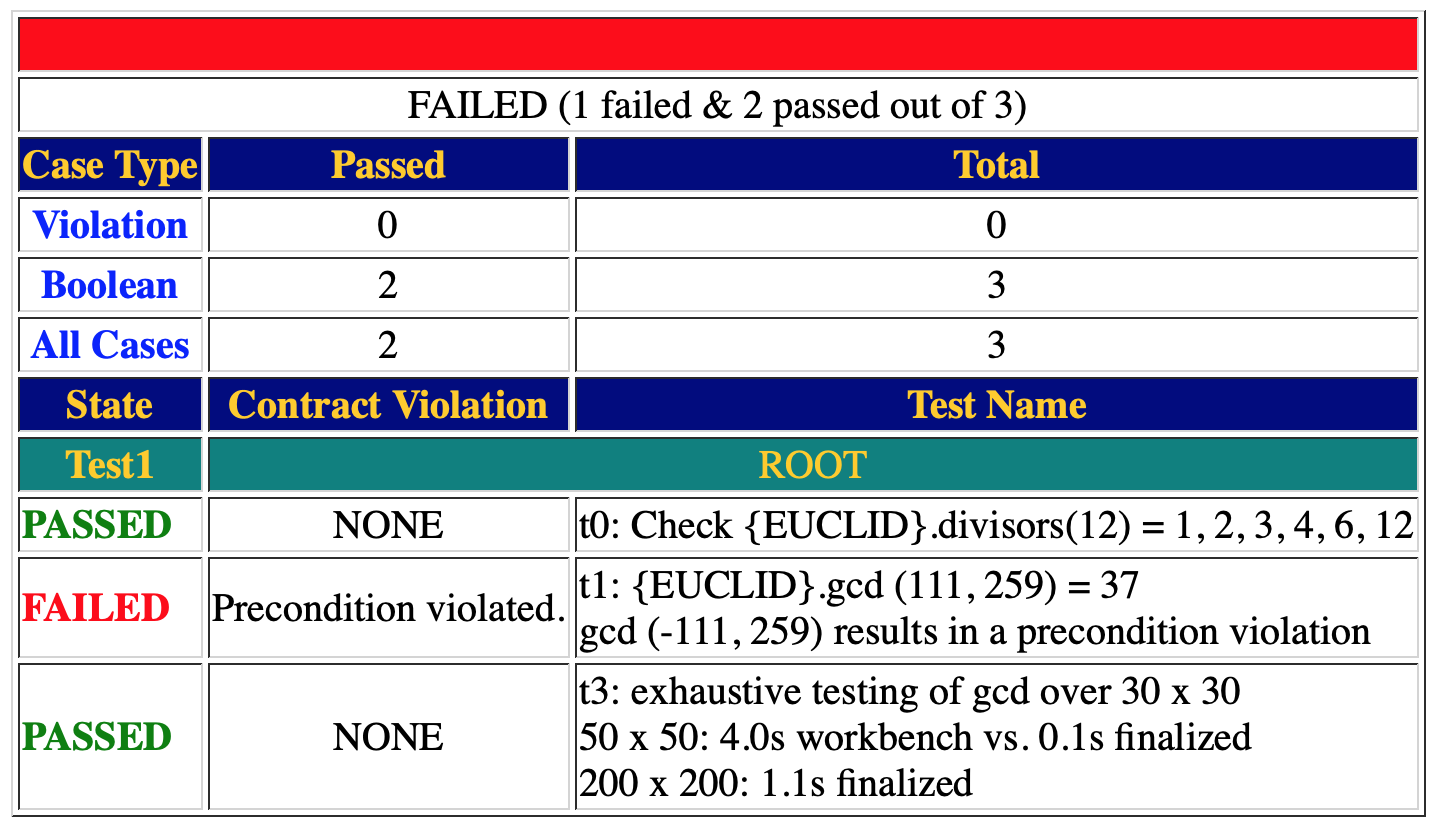
\includegraphics[width=.8\textwidth]{images/precondition-violate.png}

\subsection{Termination and Correctness} 

But we still need to prove that in the case the client makes a legal call, the GCD query terminates,  and terminates with the correct result (i.e. satisfies the specification).

To prove termination and correctness, we must provide the implementation with a loop \textbf{variant} (i.e. $x +y$) and \textbf{loop invariant} (i.e. $gcd\_spec(x,y) = gcd\_spec(m,n)$) as shown in Fig.~\ref{fig:gcd}.

%%%%%%%%%%%%%%%%%%%%%%%%%%%%%%%%%%%%%%%%%%%%%%%%%%%%%%%%%%%%%%%%%
\begin{figure}[!htb]
\begin{framed}
\caption{Specification and implementation of the GCD query in Eiffel}
\label{fig:gcd}
\lstset{language=eiffel}    
\begin{lstlisting} 
gcd(m, n: INTEGER): INTEGER
		-- return the greatest common divider of $m$ and $n$
	require
		$m \geq 1 \land n \geq 1$ -- at least should not be zero
	local
		x, y: INTEGER
	do
		from
			x := m; y := n
		invariant 
			inv: gcd_spec(x,y) = gcd_spec(m,n)
		until
			x = y
		loop
			if x < y then
				y := y - x
			else -- $ x < y$
				x := x - y
			end
		variant x + y
		end
		check x = y and x = gcd_spec(m,n) end
		Result := x
	ensure 
			Result = gcd_spec(m,n)
	end
\end{lstlisting} 
\end{framed}
\end{figure}

%%%%%%%%%%%%%%%%%%%%%%%%%%%%%%%%%%%%%%%

\section{Proof of Termination and Correctness}
%%%%%%%%%%%%%%%%%%%%%%%%%%%%%%%%%%%%%%%%%%%%%

There are five proof obligations that must be discharged to prove that the loop terminates, and terminates correctly. 

\subsection{ Prove that $P$ is true initially}
	
\begin{calculation}
	wp(a:=0, P)
\hint{=}{defn. of weakest precondition for assignment}
	P [a := 0]
\hint{=} {defn. of $P$}
	(0 \leq a^2 \leq n)[a := 0]
\hint{=} {substituting all free occurrences of $a$ in $P$ by zero}
	0 \leq 0^2 \leq n
\hint{=}{$0 \leq 0^2 \leq n \1\equiv 0 \leq  n$ and Leibniz}
	0 \leq n
\end{calculation}

%%%%%%%%%%%%%%%%%%%%%%%%%%%%%%%%%%%%%%%
\section{Prove that each iteration of the loop preserves $P$}

Must show that: $\{P \land B\}\; a := a + 1 \;\{P\}$, where $B$ is the guard of the loop. 
	
\begin{calculation}
	P \land B
\hint{=} {definition pf $P$ and $B$}
	(0 \leq a^2 \leq n) \land ((a+1)^2 \leq n)
\hint{\Rightarrow}{weakening}
	0 \leq (a+1)^2 \leq n
\hint{=}{by substitution}
	(0 \leq a^2 \leq n)[a := a+1]
\hint{=}{defn  of $P$}
	P [a := a+1]
\hint{=} {defn. of wp}
	wp(a := a +1, P)
\end{calculation}

%%%%%%%%%%%%%%%%%%%%%%%%%%%%%%%%%%%%%%%

\section{Prove that $P \land \lnot B \limp R$, i.e. the postcondition} 
	
\begin{calculation}
	P \land \lnot B
\hint{=}{defn. of $P$ and $B$}
	 (0 \leq a^2 \leq n) \land \lnot ((a+1)^2 \leq n)
\hint{=}{arithmetic and negation}
	0 \leq a^2 \leq n) \land ((a+1)^2 > n)
\hint{=}{rearranging}
	0 \leq a^2 \leq n < (a+1)^2
\end{calculation}

%%%%%%%%%%%%%%%%%%%%%%%%%%%%%%%%%%%%%%%

\section{Show that the variant $t$ is bounded from below}
 
\begin{calculation}
	P \land B
\hint{=} {definition pf $P$ and $B$}
	(0 \leq a^2 \leq n) \land ((a+1)^2 \leq n)
\hint{\Rightarrow}{weakening}
	a^2 \leq n
\hint{=}{sqrt of both sides and $n \geq 0$}
	a \leq \sqrt n
\hint{=}{arithmetic}
	\sqrt n - a \1\geq 0
\hint{=}{defn. of $t$}
	t \geq 0
\end{calculation}
%%%%%%%%%%%%%%%%%%%%%%%%%%%%%%%%%%%%%%%

\section{Show that the variant decreases in each iteration}

Must show that: $\{P \land B \land t = T_0\}\; a := a + 1 \;\{t < T_0\}$, where $B$ is the guard of the loop. 

\begin{calculation}
	wp(a := a +1, t < T_0)
\hint{=} {defn. of weakest precondition}
	(t < T_0)\;[a := a+1]
\hint{=}{defn. of $t$}
	(\sqrt n - a < T_0)\;[a := a +1]
\hint{=}{substitution}
	\sqrt n - (a+1) < T_0
\hint{=}{In the precondition, $t \1= T_0 \1= \sqrt n - a $}
	\sqrt n - (a+1) < \sqrt n - a
\hint{=}{Arithmetic and Leibniz}
	(\sqrt n - a) -1 < \sqrt n - a
\hint{=}{Arithmetic $x - 1 < x$ for any $x$}
	true
\end{calculation}


\end{document}
